%Compiler: LuaLatex
%If compilation does not work, please change the compiler.
\documentclass[11pt,a4paper, english]{article}

%Using Preamble.tex of paulgp/draft-tex
%https://github.com/paulgp/draft-tex

\usepackage[top=0.8in, bottom=0.78in, left=0.87in, right=0.87in]{geometry}
\usepackage{setspace}
\usepackage[T1]{fontenc}
\usepackage{times}
\usepackage{booktabs}
\usepackage{rotating}
\usepackage{graphicx}
\usepackage[section]{placeins} %Placeins.sty keeps floats `in their place', preventing them from floating past a "\FloatBarrier" command into another section.  To use it, declare "\usepackage{placeins}" and insert "\FloatBarrier" at places that floats should not move past, perhaps at every "\section".  
\usepackage[large, bf]{caption}
\usepackage[FIGTOPCAP]{subfigure}
\usepackage{pdfpages}
\usepackage{palatino}
\usepackage{pdflscape}
\usepackage{textcomp}
\usepackage{longtable}
\usepackage{nicefrac}
\usepackage{adjustbox}	% to adjust the size of objects to fit into a page
\usepackage[hyphens]{url}


\usepackage{natbib}
\bibpunct{(}{)}{;}{a}{,}{,}

\def\citeapos#1{\citeauthor{#1}'s (\citeyear{#1})}

\doublespacing

\usepackage{amsmath, amsfonts, amssymb, amsthm}

\usepackage{mathpazo} %Use Palotino fonts
\parskip 0ex  %Vertical distance between paragraphs, in "ex"s
\parindent 20pt


\usepackage[pdftex]{hyperref}
\hypersetup{colorlinks, citecolor=blue, filecolor=blue, linkcolor=blue, urlcolor=blue}



%\usepackage{subcaption} % for figures


\newtheorem{theorem}{Theorem}
\newtheorem{lemma}{Lemma}
\newtheorem{proposition}{Proposition}
\newtheorem{corollary}{Corollary}
\newtheorem{prediction}{Prediction}
\newtheorem{case}{Special Case}

\newenvironment{proofAlt}[1][Proof]{\begin{trivlist}
\item[\hskip \labelsep {\bfseries #1}]}{\end{trivlist}}
\newenvironment{definition}[1][Definition]{\begin{trivlist}
\item[\hskip \labelsep {\bfseries #1}]}{\end{trivlist}}
\newenvironment{example}[1][Example]{\begin{trivlist}
\item[\hskip \labelsep {\bfseries #1}]}{\end{trivlist}}

\newenvironment{remark}[1][Remark]{\begin{trivlist}
\item[\hskip \labelsep {\bfseries #1}]}{\end{trivlist}}
\def\urltilda{\kern -.15em\lower .7ex\hbox{\~{}}\kern .04em}

\renewcommand{\thesubfigure}{(\Alph{subfigure})}


%%%%%%%%%%%%%%%%%%%%%%%%%%%%%%%%%%
% SPACING
%%%%%%%%%%%%%%%%%%%%%%%%%%%%%%%%%%

\usepackage{titlesec}

\titlespacing*{\section}{0pt}{1.5ex plus 1ex minus .2ex}{0.8ex plus .2ex}
\titlespacing*{\subsection}{0pt}{1.2ex plus 1ex minus .2ex}{0.8ex plus .2ex}
\usepackage{appendix}
% Decimal align 
\usepackage{dcolumn}
\newcolumntype{d}[0]{D{.}{.}{5}}

% Spaces in file path
\usepackage{graphicx}
\usepackage[space]{grffile}

%%%%%%%%%%%%%%%%%%%%%%%%%%%%%%%%%%
% Tables
\usepackage{threeparttable}

%%%%%%%%%%%%%%%%%%%%%%%%%%%%%%%%%%
% Packages for Tables generated by R ----
\usepackage{tabularray}
\usepackage{booktabs} 
\usepackage{longtable}
\usepackage{array}
\usepackage{multirow}
\usepackage{wrapfig} % if necessary
\usepackage{float}
\usepackage{colortbl} % if necessary
\usepackage{pdflscape}
\usepackage{tabu}
\usepackage{threeparttable}
\usepackage{threeparttablex}
\usepackage[normalem]{ulem}
\usepackage{makecell}
\usepackage{xcolor} % if necessary
\usepackage{siunitx}
\usepackage{comment}
% -----------------------------------------

%%%%%%%%%%%%%%%%%%%%%%%%%%%%%%%%%%%%%%%%%%%%%%%%%%%%%%%%%%%%%

%%%%%%%%%%%%%%%%%%%%%%%%%%%%%%%%
%For long notes
%https://www.hargaden.com/enda/long-or-multiple-line-notes-in-esttab-with-automatic-wrapping/
\newcommand{\tabnotes}[2]{\bottomrule \multicolumn{#1}{@{}p{0.70\linewidth}@{}}{\footnotesize #2 }\end{tabular}\end{table}} 
%%%%%%%%%%%%%%%%%%%%%%%%%%%%%%%%


\begin{document}

\noindent
\textbf{{\Large Online Appendix}}\\
Michael Ryan and Ayumu Tanaka
``Anchored Abroad: Sunk Costs, Asset Specificity, and Japanese Affiliate Exit from Brexit Britain"

%\vspace{1cm}


%%%%%%%%%%%%%%%%%%%%%%%%%%%%%%%%%%%%%%%%%%%%%%%%%%%%%%%%%%%%%%%%
\setcounter{page}{1}
\setcounter{table}{0}
\renewcommand{\thetable}{X\arabic{table}}
\setcounter{figure}{0}
\renewcommand{\thefigure}{X\arabic{figure}}
\setcounter{section}{0}
\renewcommand{\thesection}{X\arabic{section}}
%%%%%%%%%%%%%%%%%%%%%%%%%%%%%%%%%%%%%%%%%%%%%%%%%%%%%%%%%%%%%%%%

\section{Affiliate size of exiting affiliates}\label{size}

Figure \ref{fig:affsize} presents the number of exiting affiliates by size category. While exits are most concentrated among the smallest-size affiliates, a considerable number of exits are also observed in the medium- and large-size categories.


%%%%%%%%%%%%%%%%%%%%%%%%%%%%%%%%%%%%%%%%%%%%%%%%%%%%%%%%
\begin{figure}[ht]
\begin{center}
  \begin{minipage}[b]{0.9\linewidth}
    \centering
    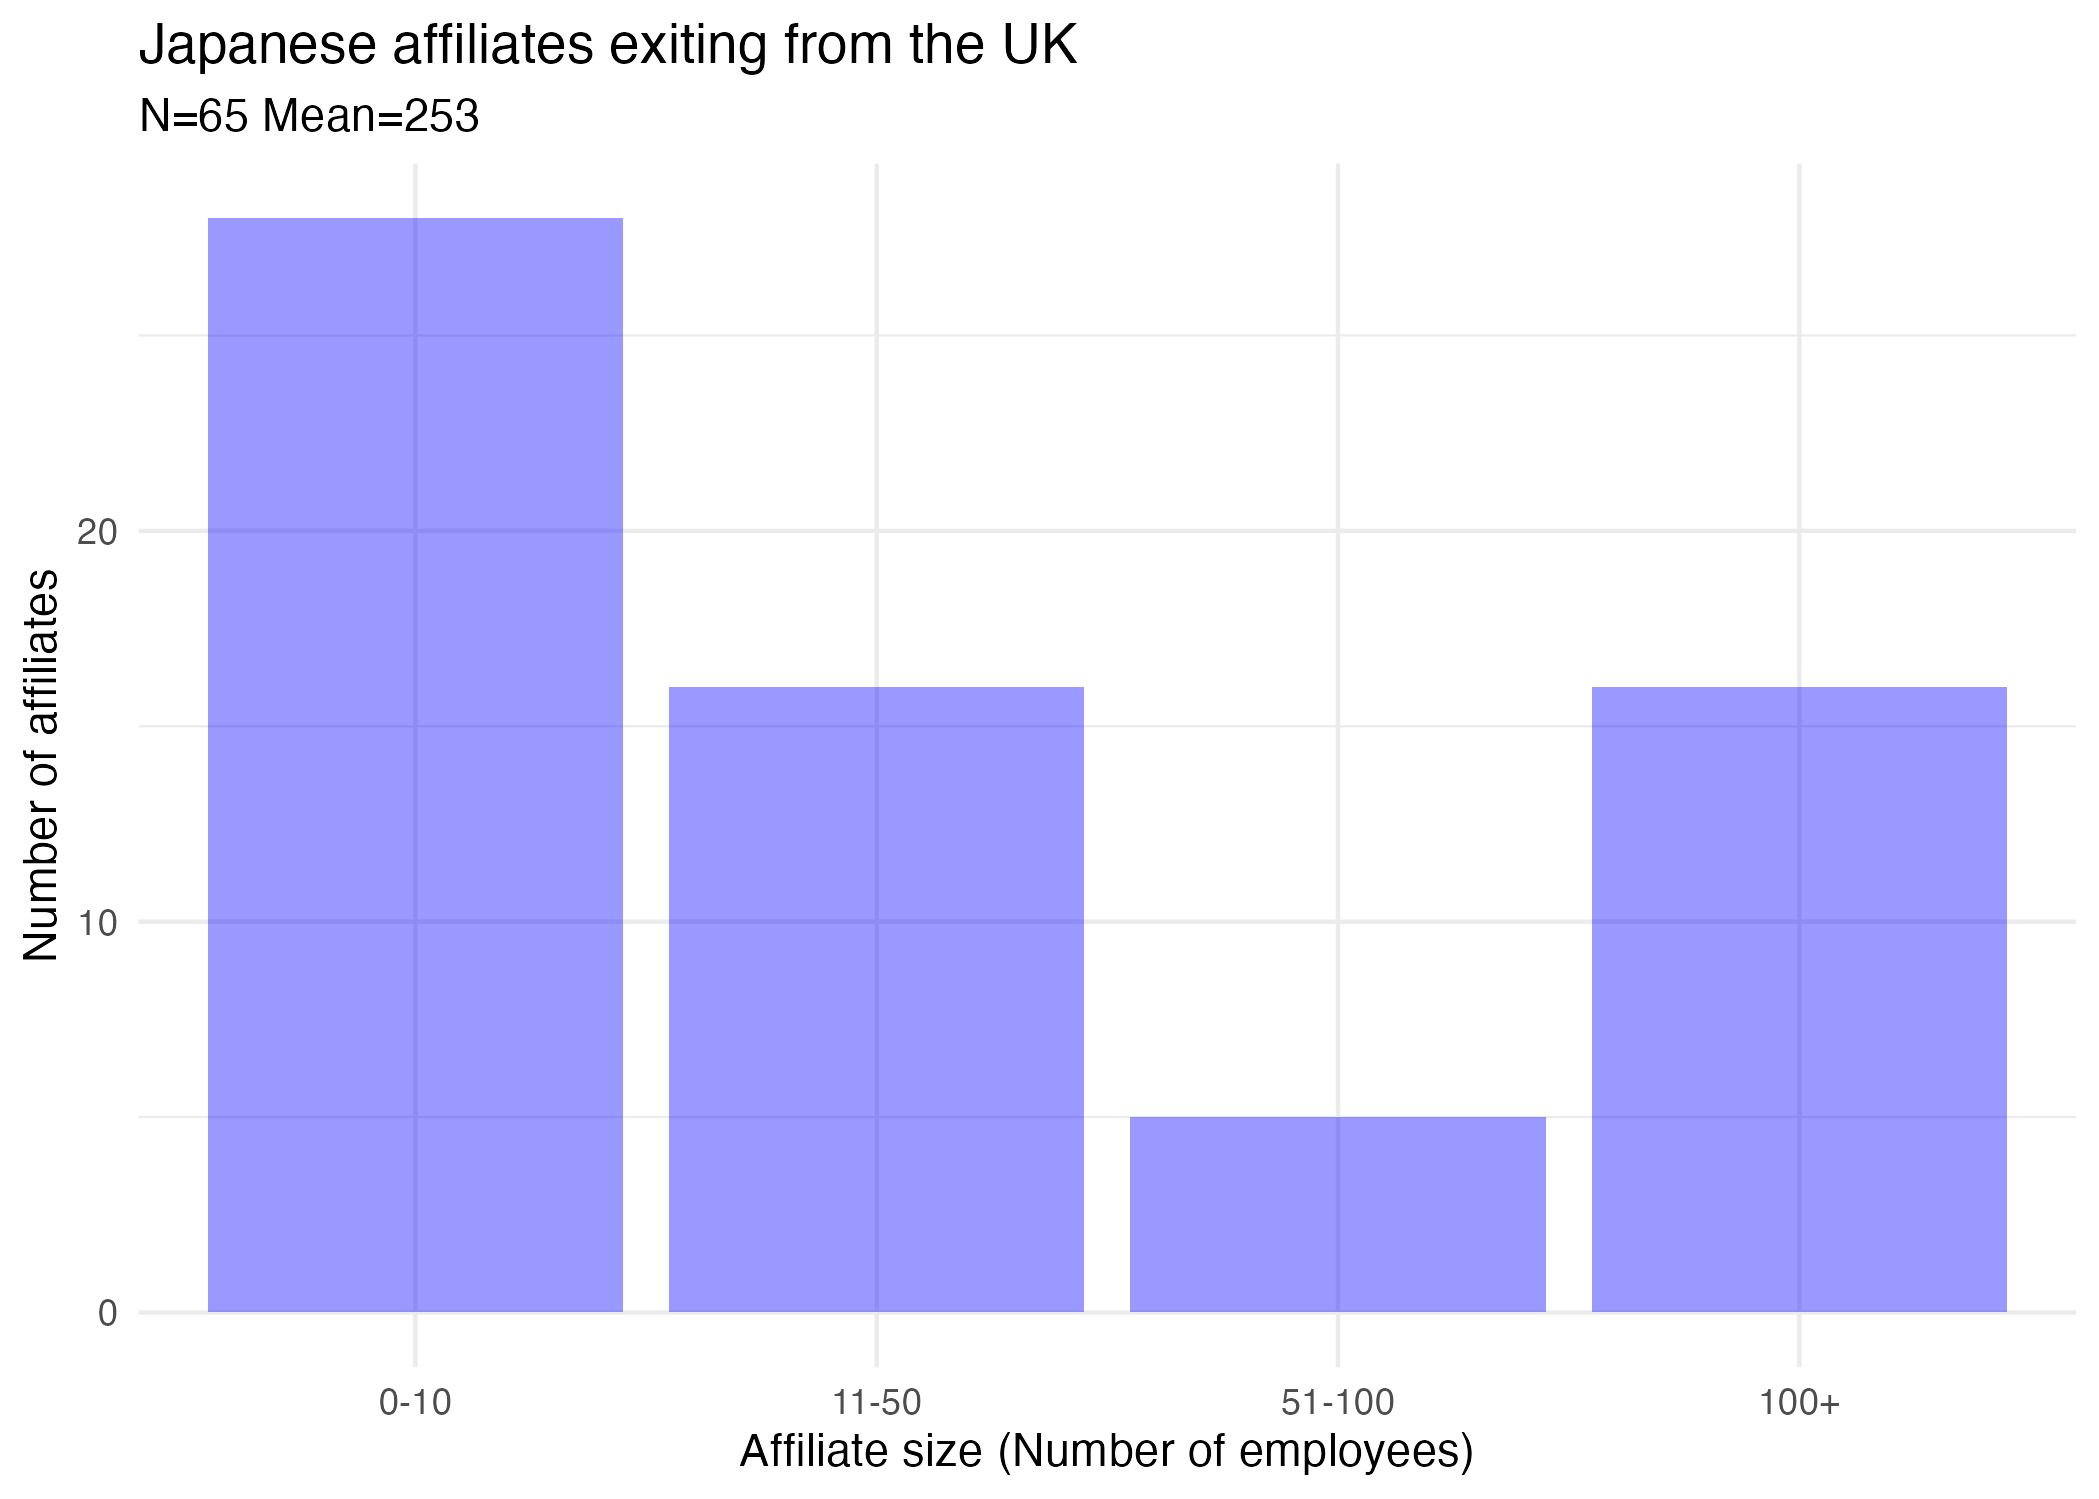
\includegraphics[keepaspectratio, scale=0.5]{FigX1.png}
  \end{minipage}
  \caption{Affiliate size of exiting affiliates}
    \label{fig:affsize}

\end{center}

\footnotesize
\emph{Source:} Authors' compilation based on Toyo Keizai's OJC data.\\
\emph{Note:} The figure presents the number of affiliates by size category, excluding those without employee data. In contrast, the regression analysis in the main text includes these affiliates by imputing missing employee numbers.
 
\end{figure}
% Fig2a_X1_X3.Rmd
%%%%%%%%%%%%%%%%%%%%%%%%%%%%%%%%%%%%%%%%%%%%%%%%%%%%%%%%



\section{Average ownership ratio}\label{ratio}

Figure \ref{fig:ratio} presents the average ownership ratio by country group. The UK exhibits a higher average ownership ratio than high-income EU member countries. The figure also indicates an upward trend in ownership ratios in both groups. However, it does not provide clear evidence that the gap between the UK and high-income EU member countries is widening.


%%%%%%%%%%%%%%%%%%%%%%%%%%%%%%%%%%%%%%%%%%%%%%%%%%%%%%%%
\begin{figure}[ht]
\begin{center}
  \begin{minipage}[b]{0.9\linewidth}
    \centering
    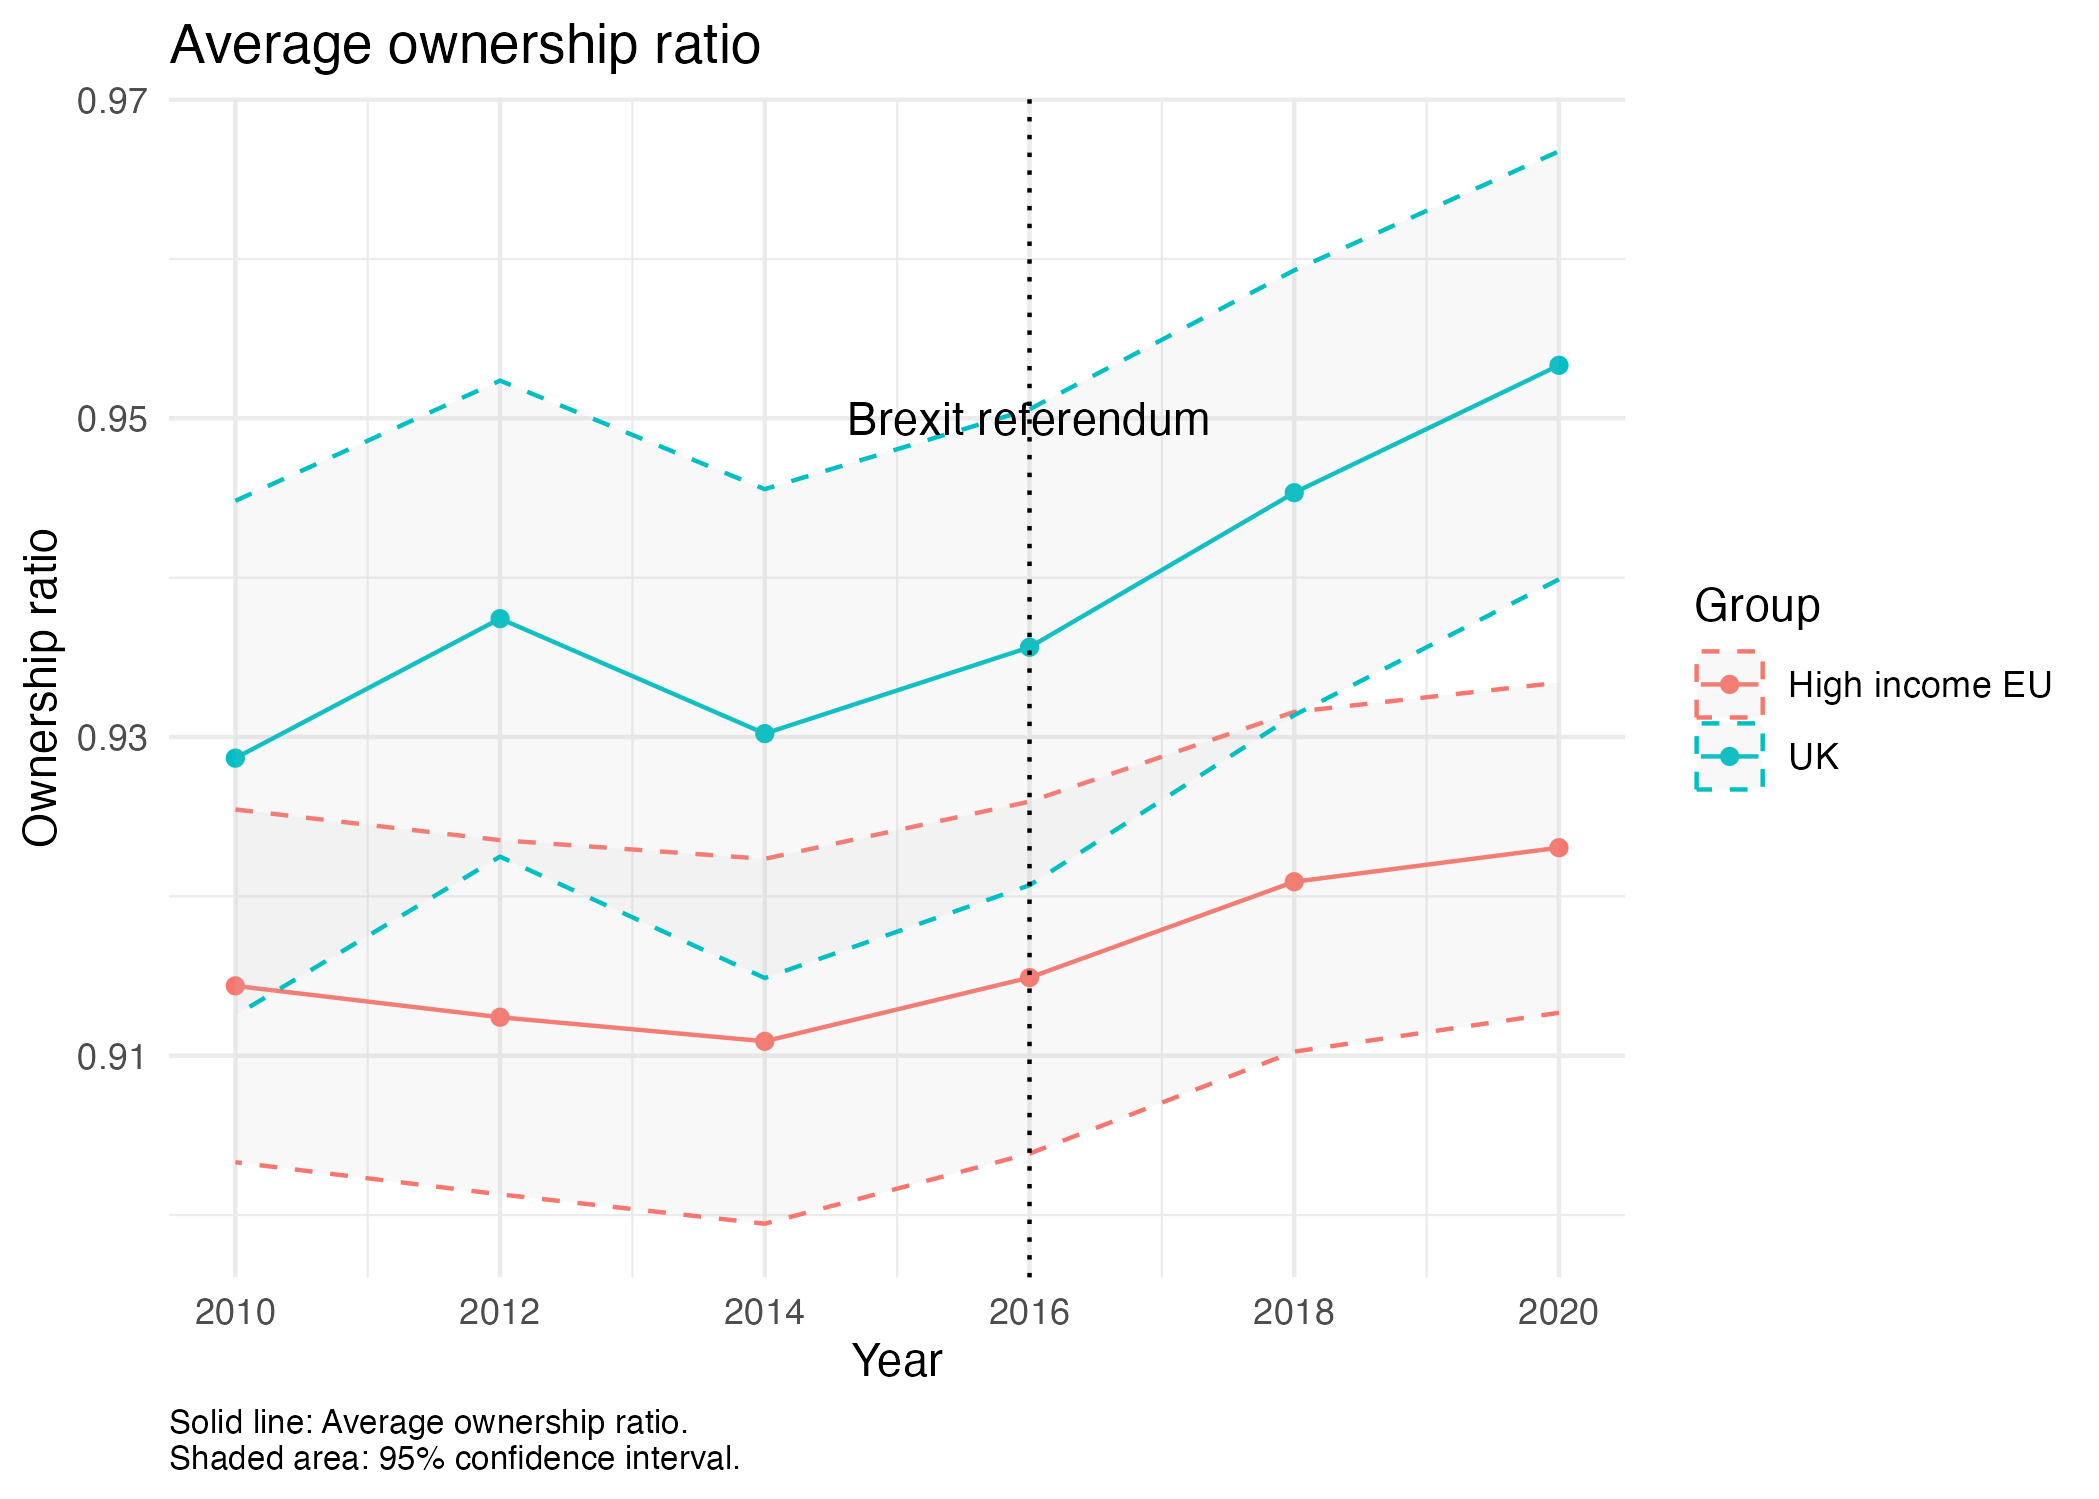
\includegraphics[keepaspectratio, scale=0.6]{FigX2.png}
    
%    \subfigure{(a) High income EU}


  \end{minipage}
  \caption{Average ownership ratio by country group}
    \label{fig:ratio}

\end{center}

\footnotesize
\emph{Source:} Authors' compilation based on Toyo Keizai's OJC data.\\
\emph{Note:} The figure presents the evolution of average ownership by country group, along with 95\% confidence intervals. It compares the average ownership ratio in high-income EU member countries with that in the UK.

\end{figure}
% Fig1_X2.Rmd
%%%%%%%%%%%%%%%%%%%%%%%%%%%%%%%%%%%%%%%%%%%%%%%%%%%%%%%%


\section{Number of firms and affiliates exiting the UK by sector}\label{sector}

Figure \ref{fig:sector} shows the number of firms and affiliates exiting the UK by sector. It indicates that firm exits are relatively concentrated in the manufacturing sector, whereas affiliate exits are more prevalent in the services sector.


%%%%%%%%%%%%%%%%%%%%%%%%%%%%%%%%
\begin{figure}[ht]
    \centering
    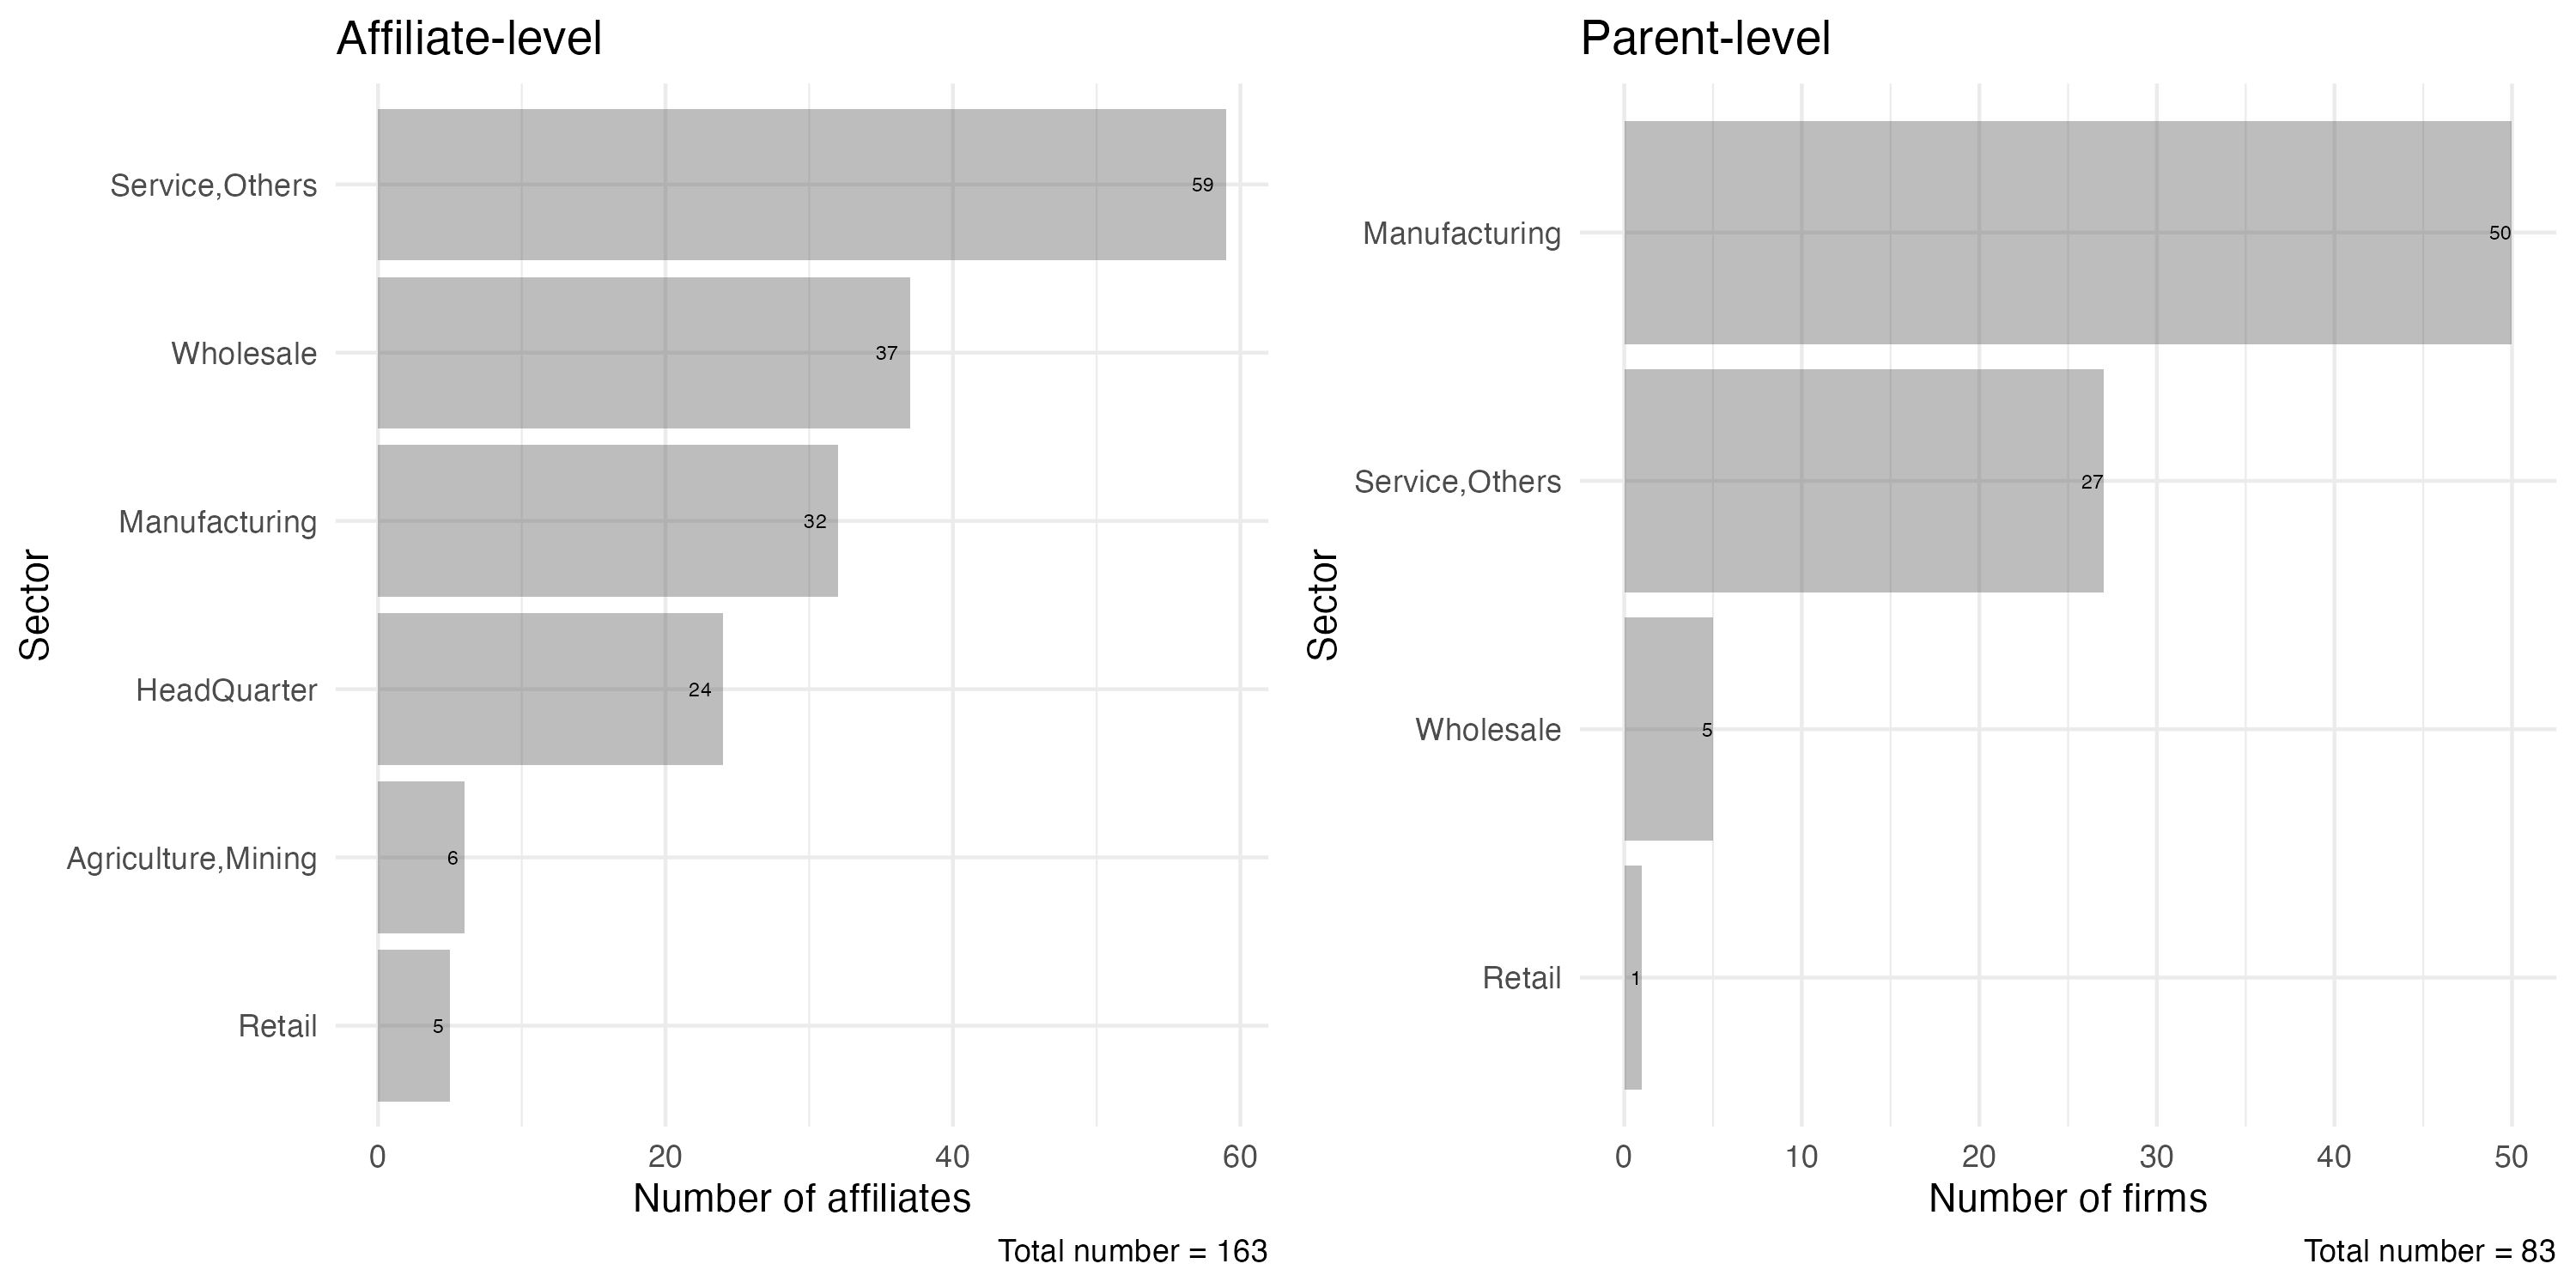
\includegraphics[width=0.9\linewidth]{FigX3.png}
    \caption{Number of firms and affiliates exiting the UK by sector: 2016--2020}
    \label{fig:sector}
\end{figure}
% Fig2a_X1_X3.Rmd
%%%%%%%%%%%%%%%%%%%%%%%%%%%%%%%%


\section{Kaplan--Meier survival plots}
While Figure 2 of the main text suggests no significant impact of Brexit on exit, we wish to more robustly examine this data. To begin, we employ Kaplan-Meier estimation to study Japanese exits from the UK. This method enables us to assess the survival rates of different affiliate cohorts categorized by distinct characteristics. In this case, affiliate location is the distinct characteristic, as we utilize affiliate location data from the OJC to compare the survival rates of Japanese affiliates in the UK with those in the remaining EU member countries. Figure \ref{fig:KM} illustrates the Kaplan-Meier estimates for both groups from 1990 to 2021. In the figure, year 0 represents affiliate birth, with firms still in existence in 2021 having (right-censored) ages at 31 years. Both curves exhibit the expected downward path dependence, indicating declining affiliate survival likelihood (or increased exit likelihood of exit) as affiliates age. Note that the curve representing UK-based affiliates lies below that for the EU-based affiliates. While this suggests a higher probability of exit, the figure suggests that there is not much difference between the two groups. In fact, results from a Mantel-Cox log-rank test indicate a p-value of 0.1, confirming no significant survival difference for Japanese affiliates in our two groups.  

%%%%%%%%%%%%%%%%%%%%%%%%%%%%%%%%%%%%%%%%%%%%%%%%%%%%%%%%
\begin{figure}[ht]
    \begin{minipage}{.95\linewidth}
    \begin{center}
    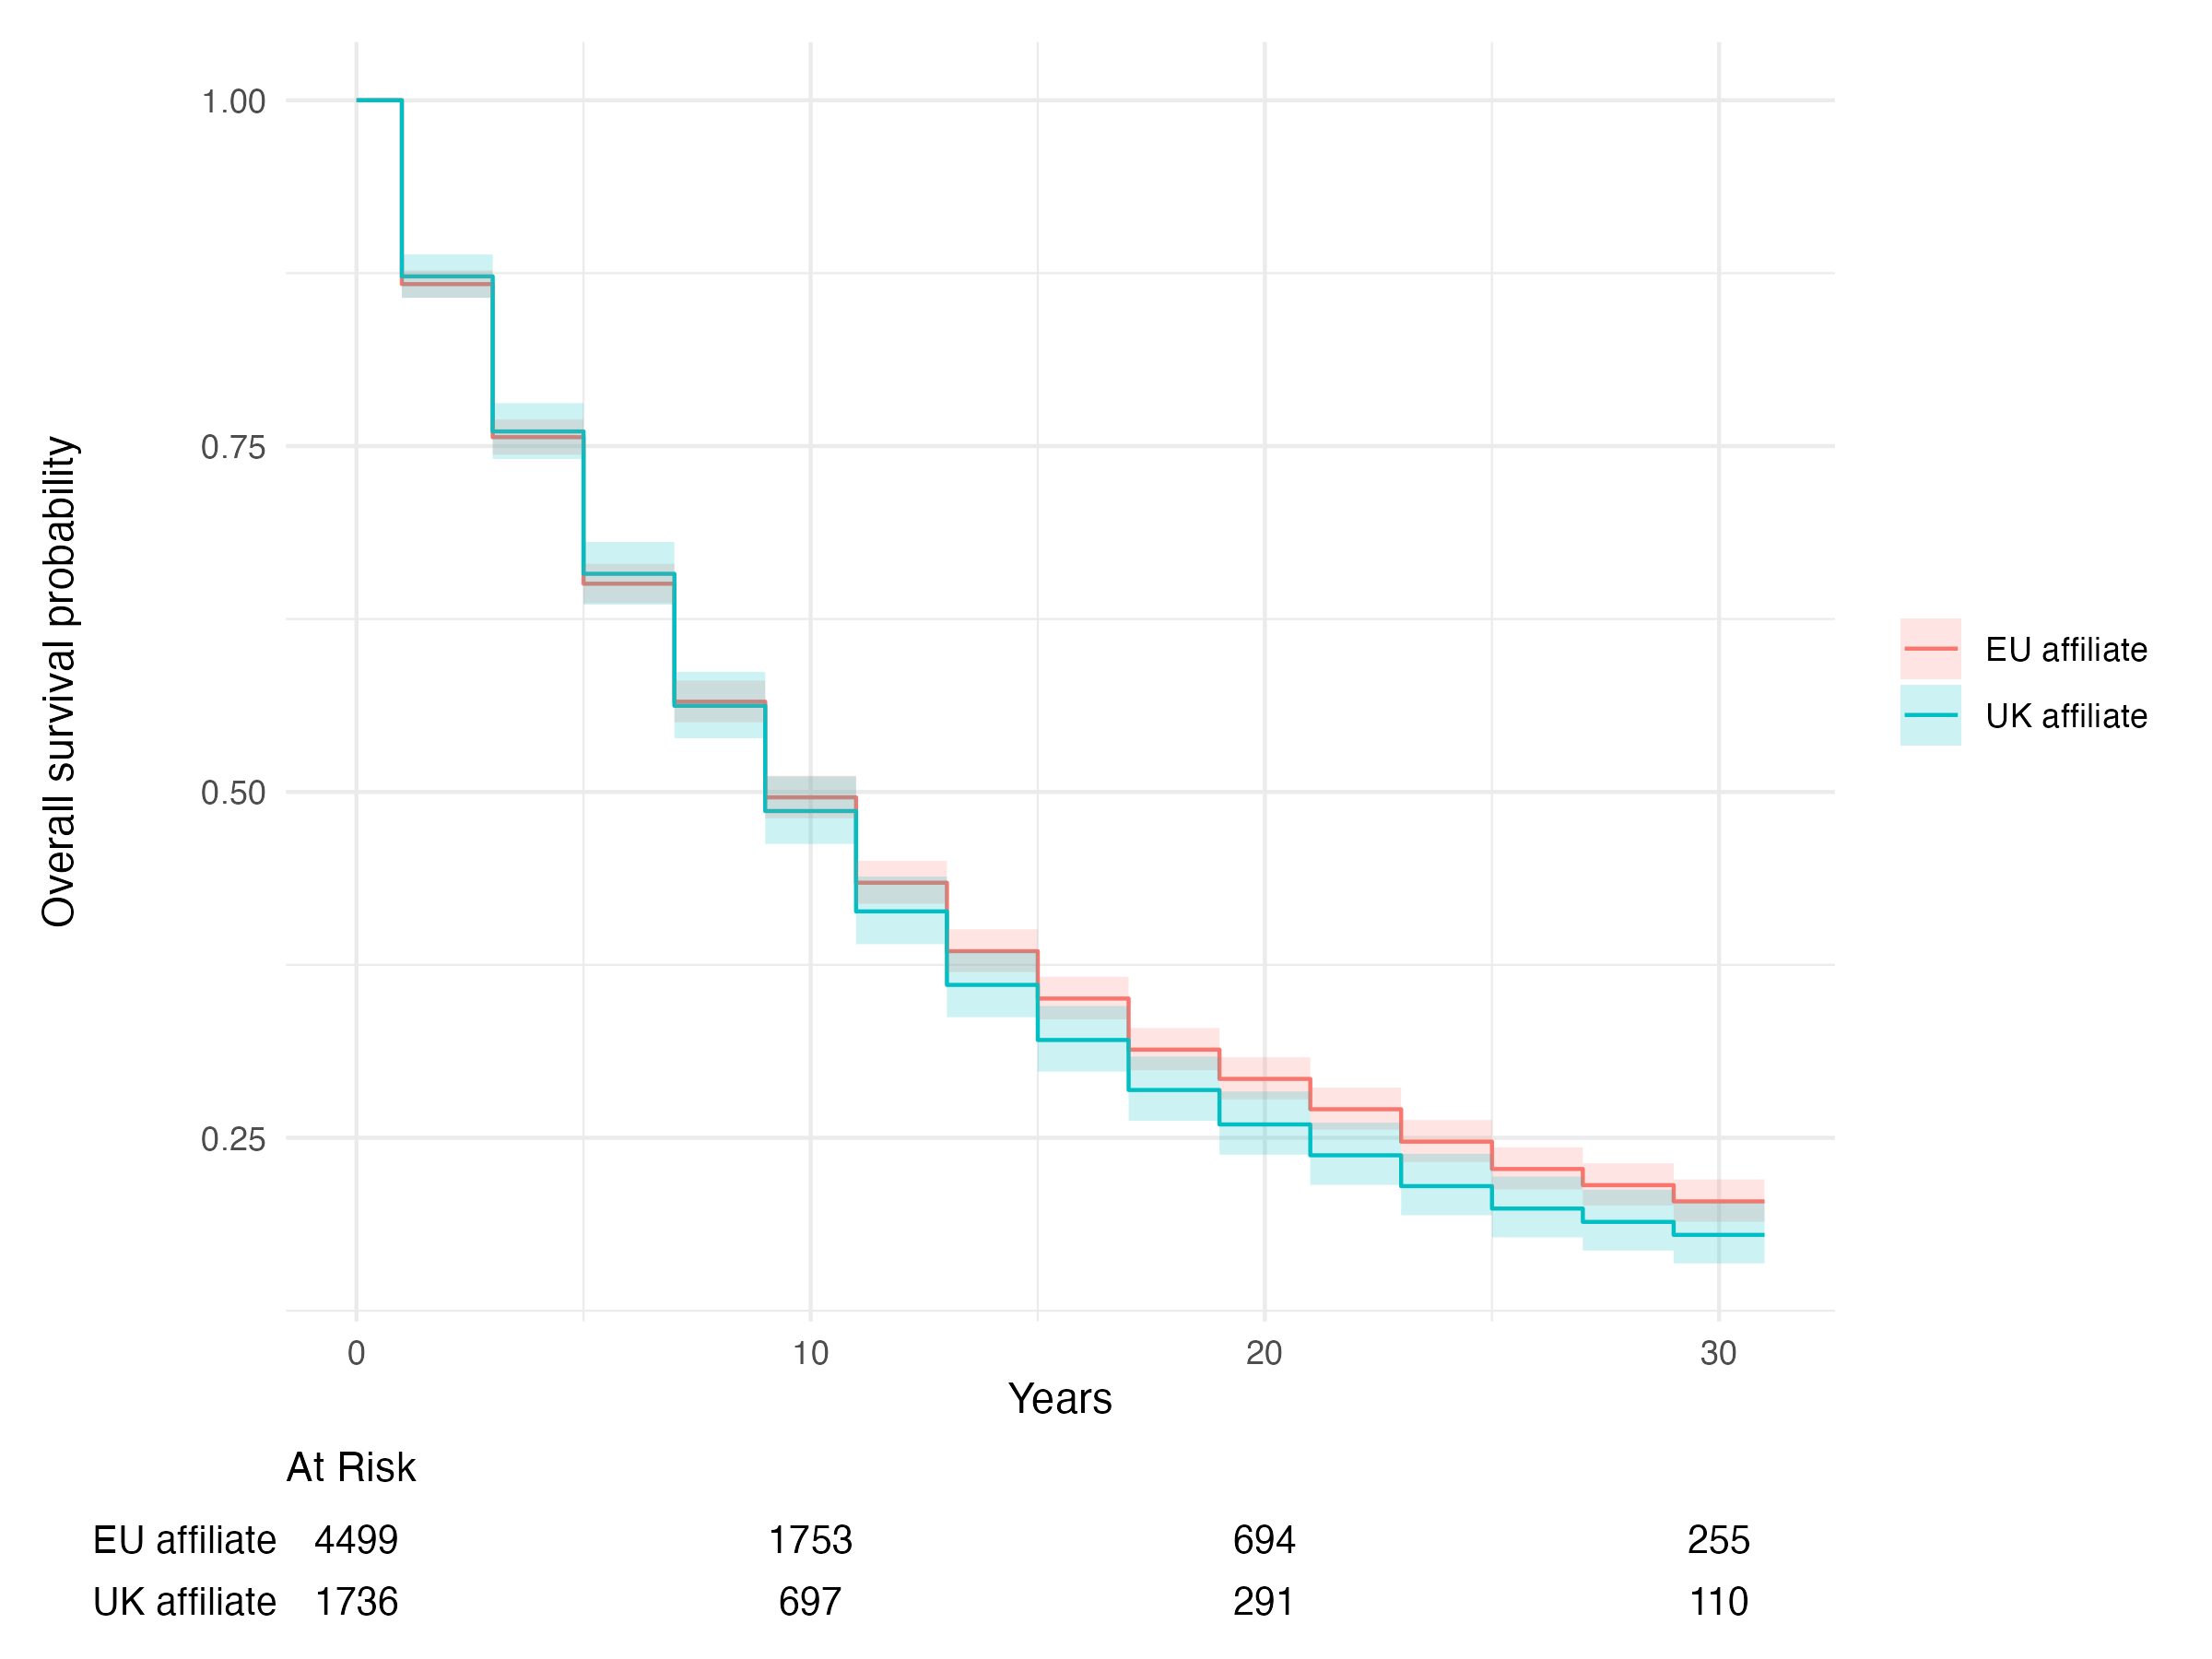
\includegraphics[width=0.7\linewidth]{FigX4.png}
    \caption{Kaplan--Meier survival estimates: UK versus EU member countries}
    \label{fig:KM}
    \end{center}

\footnotesize
\emph{Source:} Authors' compilation based on Toyo Keizai's OJC data.\\
\emph{Note:} This figure compares the survival curve of Japanese affiliates in the UK and that in other EU member countries.
\end{minipage}

\end{figure}
% FigX4_TabX1_FigX5.Rmd
%%%%%%%%%%%%%%%%%%%%%%%%%%%%%%%%%%%%%%%%%%%%%%%%%%%%%%%%


\section{Cox proportional hazards model}\label{app:cox}

We use the Cox proportional hazards model \citep{cox1972regression} to explore the factors affecting affiliate exits. 

The hazard at time $t$ is assumed to be:
\begin{equation}
h(t)=h_{0}(t) \exp \left(
    \beta_{1} Brexit+
    \beta_{2} x_{2}+\cdots+
    \beta_{k} x_{k}
    \right)
\end{equation}
where $h_{0}$ is the baseline hazard and $\beta_{1},...,\beta_{k}$ are covariates. The Cox model provides estimates of coefficients $\beta_{1},...,\beta_{k}$. Our key variable, $Brexit$, takes a value of one if the host country is the UK and $t \geq 2016$.
A failure event is an exit in our analysis. Variables with hazard ratios greater than 1 are associated with a higher likelihood of exit and shorter survival time. Variables with a hazard ratio smaller than 1 are associated with a lower likelihood of exit and longer survival time.
 The estimation results in Table \ref{tab:modelsummary-aff} show that Brexit did not have a significant impact on the Japanese affiliates' survival in the UK.



%%%%%%%%%%%%%%%%%%%%%%%%%%%%%%%%
{\renewcommand\normalsize{\scriptsize}%
\normalsize 
\begin{table}
\centering
\begin{talltblr}[         %% tabularray outer open
caption={Cox regression model at affiliate-level},
label={tab:modelsummary-aff},
note{}={* p < 0.05, ** p < 0.01, *** p < 0.001},
note{ }={Hazard ratios are reported. The Cox proportional hazards model estimates them. Failure event is exit. Variables with hazard ratios greater than 1 are associated with a higher likelihood of exit and shorter survival time. Variables with a hazard ratio smaller than 1 are associated with a lower likelihood of exit and longer survival time. Host countries' fixed effects and year-fixed effects are included in the estimation. Standard errors are presented in blankets.},
]                     %% tabularray outer close
{                     %% tabularray inner open
colspec={Q[]Q[]Q[]Q[]Q[]},
hline{2}={5}{solid, black, 0.05em},
hline{3}={1-5}{solid, black, 0.05em},
hline{17}={1-5}{solid, black, 0.05em},
hline{2}={2,4}{solid, black, 0.05em, l=-0.5},
hline{2}={3}{solid, black, 0.05em, r=-0.5},
hline{1}={1-5}{solid, black, 0.1em},
hline{21}={1-5}{solid, black, 0.1em},
column{3,5}={}{halign=c},
cell{1}{1}={}{halign=c},
cell{1}{2}={c=2}{halign=c},
cell{1}{4}={c=2}{halign=c},
cell{2-20}{1}={}{halign=l},
cell{2-20}{2}={}{halign=c},
cell{2-20}{4}={}{halign=c},
}                     %% tabularray inner close
& World &  & Europe only &  \\
& (1) & (2) & (3) & (4) \\
Brexit & 1.12740 & 1.19415* & 1.27665** & 1.23179* \\
& (0.08785) & (0.09335) & (0.11977) & (0.11576) \\
Ownership ratio & 1.22022*** & 1.16762*** & 0.81130*** & 0.80571*** \\
& (0.02711) & (0.02523) & (0.05091) & (0.05082) \\
Affiliate size & 0.99997** & 0.99996** & 0.99992 & 0.99990* \\
& (0.00001) & (0.00001) & (0.00005) & (0.00005) \\
GBR & 0.93587* &  & 0.94301 &  \\
& (0.02811) &  & (0.03234) &  \\
log GDP, PPP & 1.02736*** &  & 0.94492*** &  \\
& (0.00387) &  & (0.01573) &  \\
log GDP per capita, PPP & 0.88693*** &  & 0.65414*** &  \\
& (0.00631) &  & (0.04948) &  \\
log Distance from Japan & 0.89376*** &  & 0.36058*** &  \\
& (0.00777) &  & (0.11178) &  \\
Fixed Effect: Year & YES & YES & YES & YES \\
Fixed Effect: Sector & YES & YES & YES & YES \\
Fixed Effect: Country & NO & YES & NO & YES \\
Num.Obs. & 42935 & 45132 & 6104 & 6104 \\
\end{talltblr}
\end{table}

}
% FigX4_TabX1_FigX5.Rmd
%%%%%%%%%%%%%%%%%%%%%%%%%%%%%%%%



    %\item To examine the impact of Brexit on Japanese firms' affiliate survival in the UK, we run the Cox proportional hazard model. \item Appendix \ref{app:cox} details the estimation model and results.
Figure \ref{fig:cox_aff_world} presents coefficient estimates and 95\% confidence intervals of the Cox proportional hazard model.
Models 1--4 of Figure \ref{fig:cox_aff_world} correspond to estimation results in columns (1)--(4) of Table \ref{tab:modelsummary-aff}, respectively.
Figure \ref{fig:cox_aff_world} reveals that the 95\% confidence interval of the Brexit dummy is quite large across all models, suggesting that the impact of Brexit is insignificant and heterogeneous across Japanese affiliates in the UK.
The Cox model cannot include either affiliate fixed effects or sector $\times$ year fixed effects because they lead to the failure of convergence. 
For this reason, in the main text, we use the linear probability model that includes affiliate fixed effects and year fixed effects. 
The linear probability model results are more reliable because they control for affiliate heterogeneity and time heterogeneity. However, both models indicate that the impact of Brexit is trivial.



%%%%%%%%%%%%%%%%%%%%%%%%%%%%%%%%
\begin{figure}[ht]
    \centering
    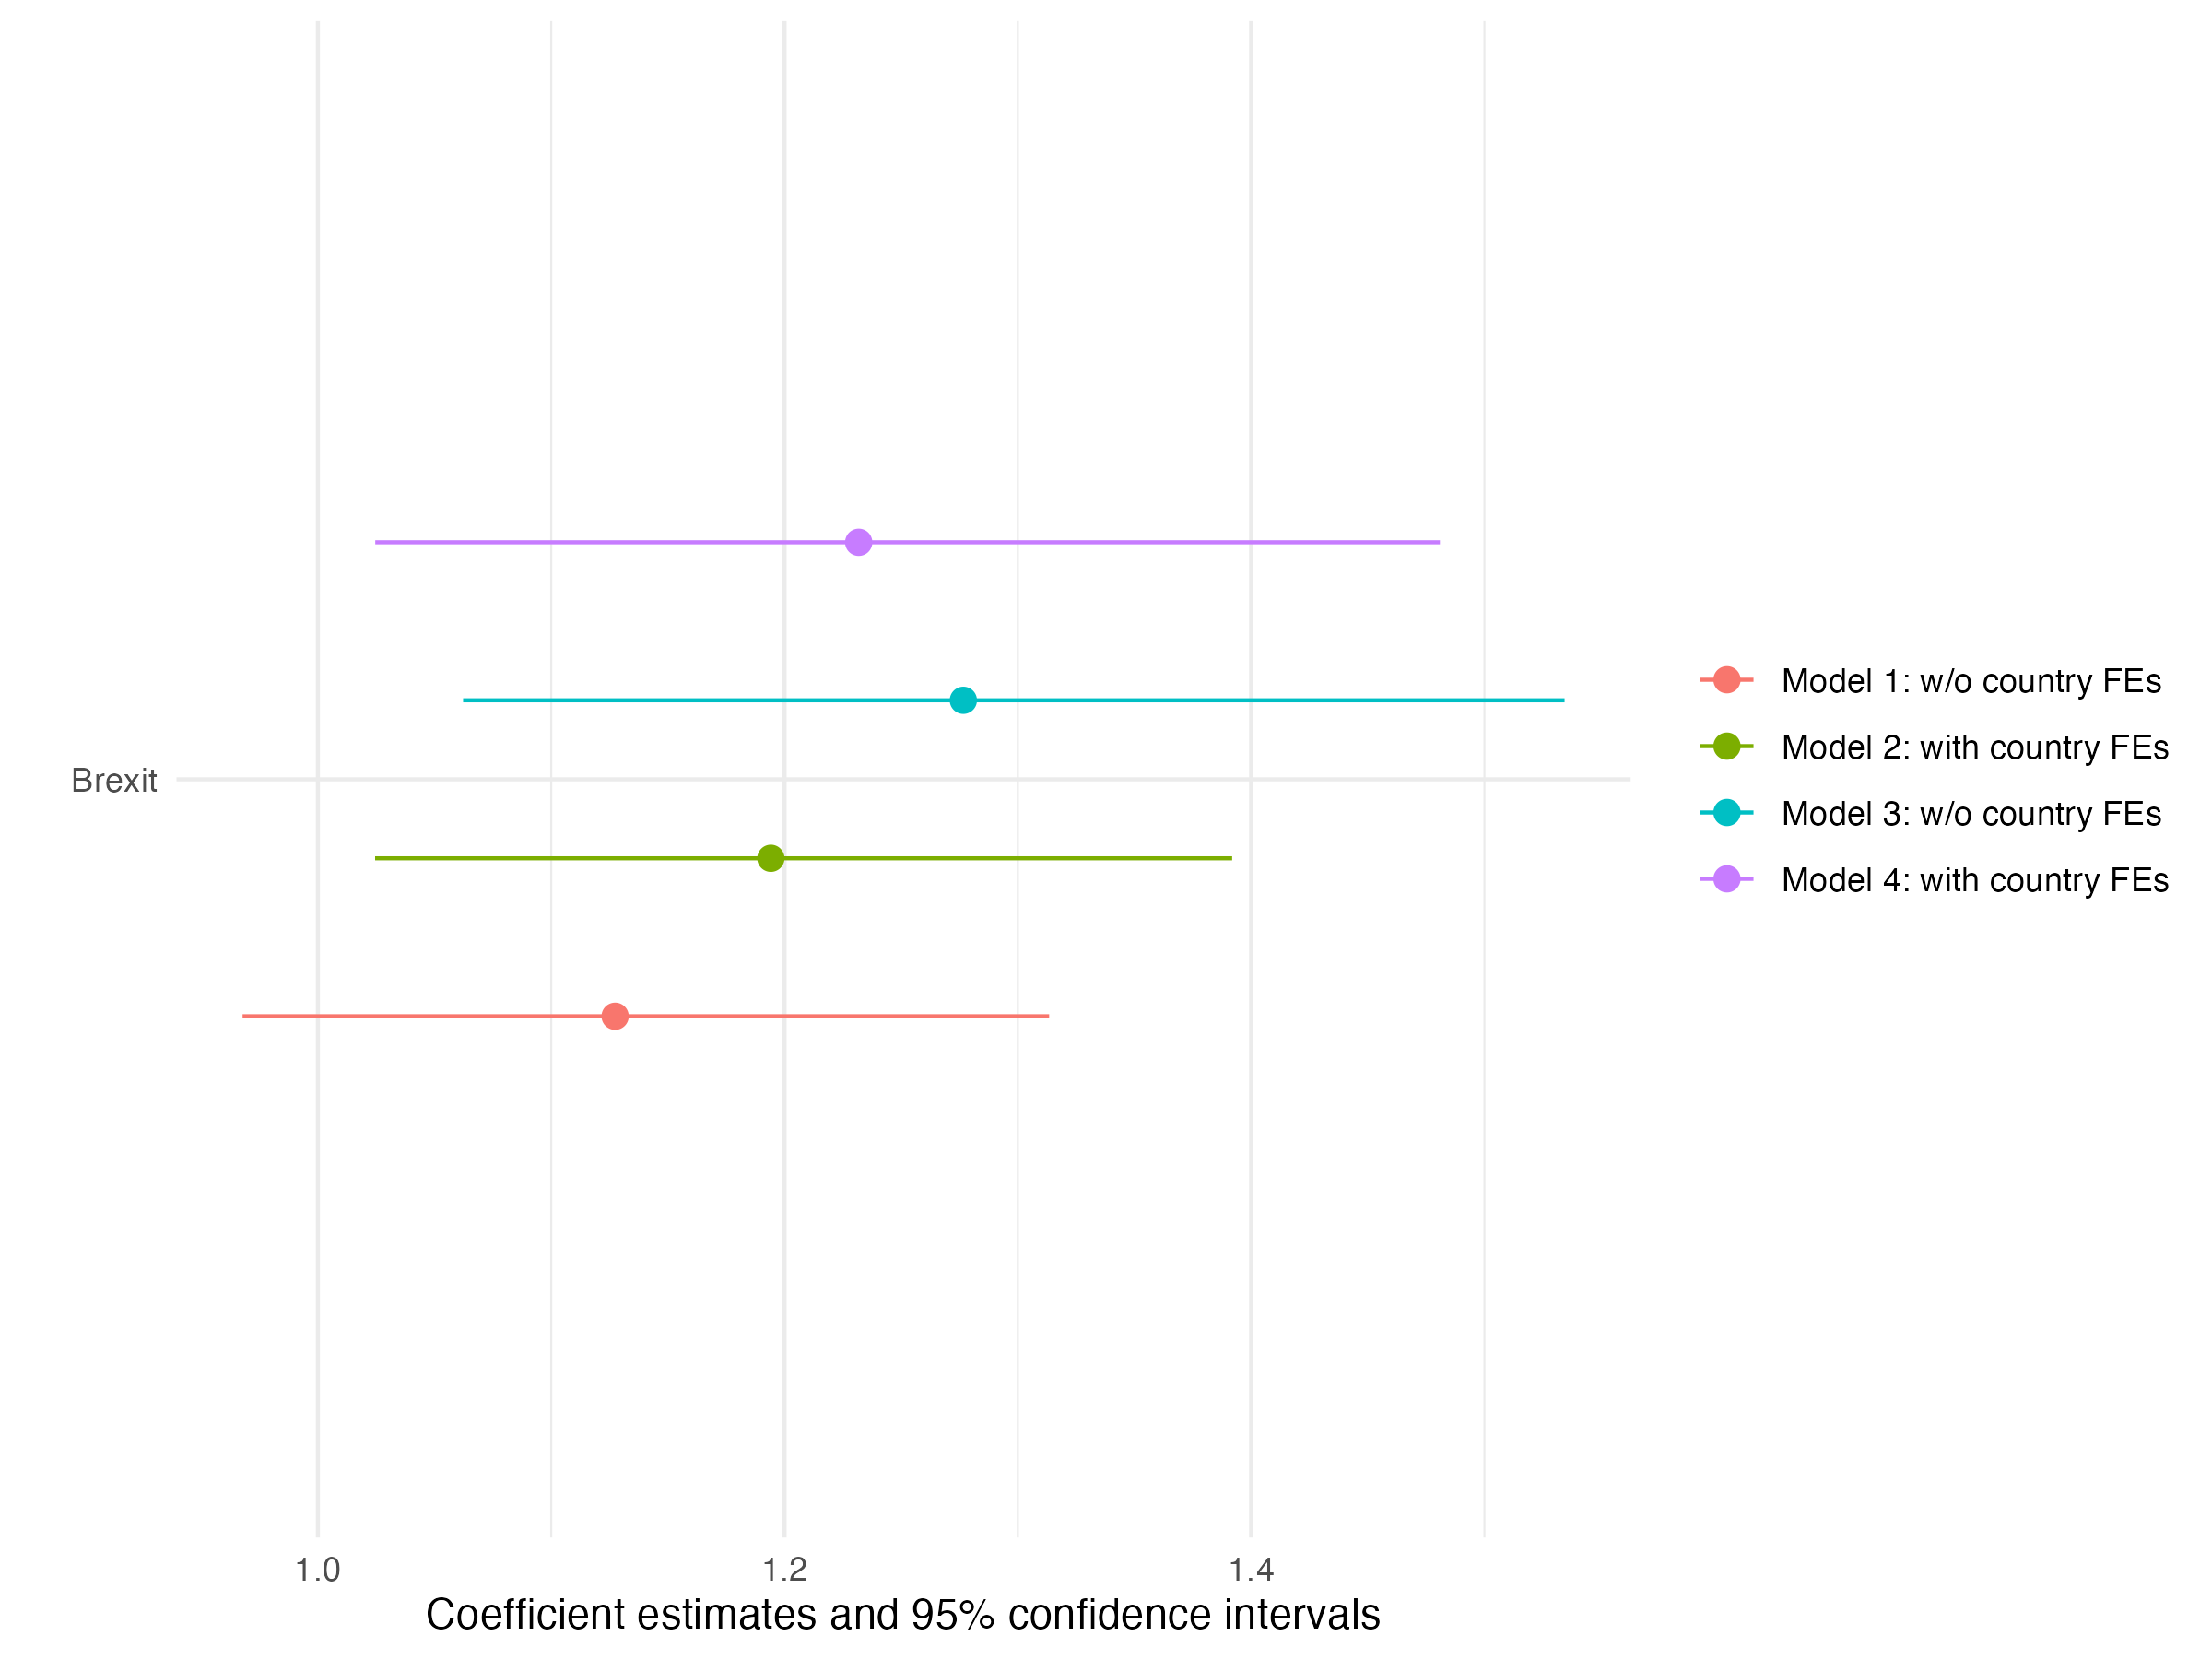
\includegraphics[width=0.6\linewidth]{FigX5.png}
    \caption{The Cox regression model's estimates of the Hazard ratio}
    \label{fig:cox_aff_world}
\end{figure}
% FigX4_TabX1_FigX5.Rmd
%%%%%%%%%%%%%%%%%%%%%%%%%%%%%%%%


\section{UK inward FDI stocks from Japan}\label{app:kox_fdi}

Figure \ref{fig:kox_fdi_stocks} provides aggregate background on the importance of Japanese investment for the UK economy. The figure uses the UIFS4 bilateral inward FDI stock database of \citet{kox2025repairing}, which reports bilateral inward FDI stocks in million US dollars. The solid line for total UK inward FDI is calculated by summing the numerical bilateral inward FDI stock cells for the UK in each year, while the Japan series corresponds to the bilateral stock for which the UK is the recipient economy and Japan is the source economy. Missing bilateral cells are not treated as zeros.

The figure shows that Japanese FDI stocks in the UK increased markedly over the 2001--2022 period. In 2016, the year of the Brexit referendum, Japanese FDI stocks in the UK were about USD 114 billion, accounting for 4.1\% of numerically reported UK inward FDI stocks. Japan was among the top ten source economies for UK inward FDI stocks throughout the sample period, and from 2014 onward it was the second-largest non-EU source economy after the United States. This aggregate evidence complements the affiliate-level analysis in the main text by showing that Japanese firms were not a marginal investor group in the UK when the referendum shock occurred.


%%%%%%%%%%%%%%%%%%%%%%%%%%%%%%%%
\begin{figure}[ht]
    \centering
    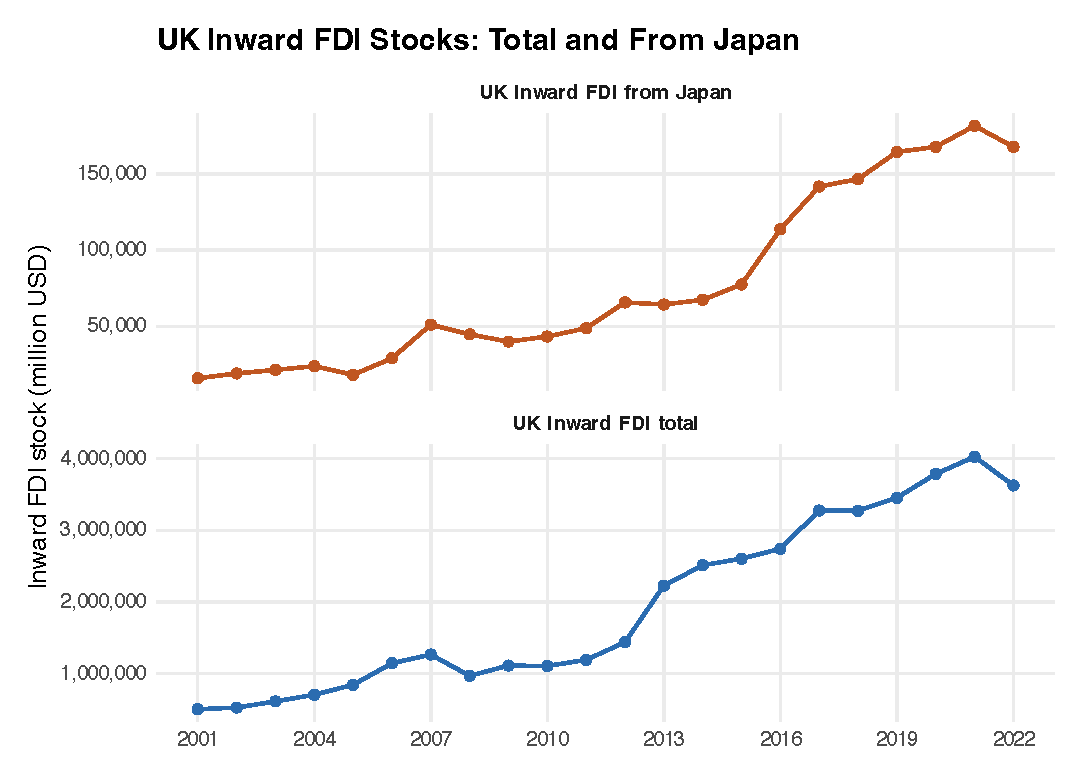
\includegraphics[width=0.75\linewidth]{FigX6.eps}
    \caption{UK inward FDI stocks: total and from Japan}
    \label{fig:kox_fdi_stocks}
\end{figure}
% FigX6.Rmd
%%%%%%%%%%%%%%%%%%%%%%%%%%%%%%%%



\bibliographystyle{aer}
\bibliography{brexit_ref}


\end{document}
